
\documentclass[12pt]{article}

% Layout.
\usepackage[top=1in, bottom=0.75in, left=1in, right=1in, headheight=1in, headsep=6pt]{geometry}

% Fonts.
\usepackage{mathptmx}
\usepackage[scaled=0.86]{helvet}
\renewcommand{\emph}[1]{\textsf{\textbf{#1}}}

% TiKZ.
\usepackage{tikz, pgfplots}
\usetikzlibrary{calc}
\pgfplotsset{compat = newest}
 
\pgfplotsset{my style/.append style={axis x line=middle, axis y line=
middle, xlabel={$x$}, ylabel={$y$}, axis equal }}

% Misc packages.
\usepackage{amsmath,amssymb,latexsym}
\usepackage{graphicx}
\usepackage{array}
\usepackage{xcolor}
\usepackage{multicol}

% Commands to set various header/footer components.
\makeatletter
\def\doctitle#1{\gdef\@doctitle{#1}}
\doctitle{Use {\tt\textbackslash doctitle\{MY LABEL\}}.}
\def\docdate#1{\gdef\@docdate{#1}}
\docdate{Use {\tt\textbackslash docdate\{MY DATE\}}.}
\def\doccourse#1{\gdef\@doccourse{#1}}
\let\@doccourse\@empty
\def\docscoring#1{\gdef\@docscoring{#1}}
\let\@docscoring\@empty
\def\docversion#1{\gdef\@docversion{#1}}
\let\@docversion\@empty
\makeatother

% Headers and footers layout.
\makeatletter
\usepackage{fancyhdr}
\pagestyle{fancy}
\fancyhf{} % Clears all headers/footers.
\lhead{\baselineskip 30pt
%\emph{\@doctitle\hfill\@docdate}
\emph{\@docdate\hfill\@doctitle}
\ifnum \value{page} > 1\relax\else\\
\emph{Name: \rule{3.5in}{1pt}\hfill \@docscoring}\fi}
\rfoot{\emph{\@docversion}}
\lfoot{\emph{\@doccourse}}
\cfoot{\emph{\thepage}}
\renewcommand{\headrulewidth}{0pt}%
\makeatother

% Paragraph spacing
\parindent 0pt
\parskip 6pt plus 1pt

% A problem is a section-like command. Use \problem{5} to
% start a problem worth 5 points.
\newcounter{probcount}
\newcounter{subprobcount}
\setcounter{probcount}{0}
\newcommand{\problem}[1]{%
\par
\addvspace{4pt}%
\setcounter{subprobcount}{0}%
\stepcounter{probcount}%
\makebox[0pt][r]{\emph{\arabic{probcount}.}\hskip1ex}\emph{[#1 points]}\hskip1ex}
\newcommand{\thesubproblem}{\emph{\alph{subprobcount}.}}

% Subproblems are an enumerate-like environment with a consistent
% numbering scheme. 
% Use \begin{subproblems}\item...\item...\end{subproblems}
\newenvironment{subproblems}{%
\begin{enumerate}%
\setcounter{enumi}{\value{subprobcount}}%
\renewcommand{\theenumi}{\emph{\alph{enumi}}}}%
{\setcounter{subprobcount}{\value{enumi}}\end{enumerate}}

% Blanks for answers in normal and math mode.
\newcommand{\blank}[1]{\rule{#1}{0.75pt}}
\newcommand{\mblank}[1]{\underline{\hspace{#1}}}
\def\emptybox(#1,#2){\framebox{\parbox[c][#2]{#1}{\rule{0pt}{0pt}}}}

% Misc.
\renewcommand{\d}{\displaystyle}
\newcommand{\ds}{\displaystyle}
\def\bc{\begin{center}}
\def\ec{\end{center}}
\def\be{\begin{enumerate}}
\def\ee{\end{enumerate}}


\doctitle{Math 251: Quiz 3}
\docdate{Feb 2, 2023}
\doccourse{UAF Calculus I}
\docversion{v-1}
\docscoring{\blank{0.8in} / 25}
\begin{document}
%\textbf{Please circle your instructor's name:} \hfill Leah Berman  \hfill   Jill Faudree\\

There are 25 points possible on this quiz. No aids (book, calculator, etc.)
are permitted.  {\bf Show all work for full credit.}

\begin{enumerate}
\item (10 points) The function $H(x)$ has domain $(-5,\infty)$ and has a vertical asymptote at $x=-5.$ Use the graph of $H(x)$ to answer each question below. If the limit is infinite, indicate that with $\infty$ or $-\infty.$ \\

\begin{center}
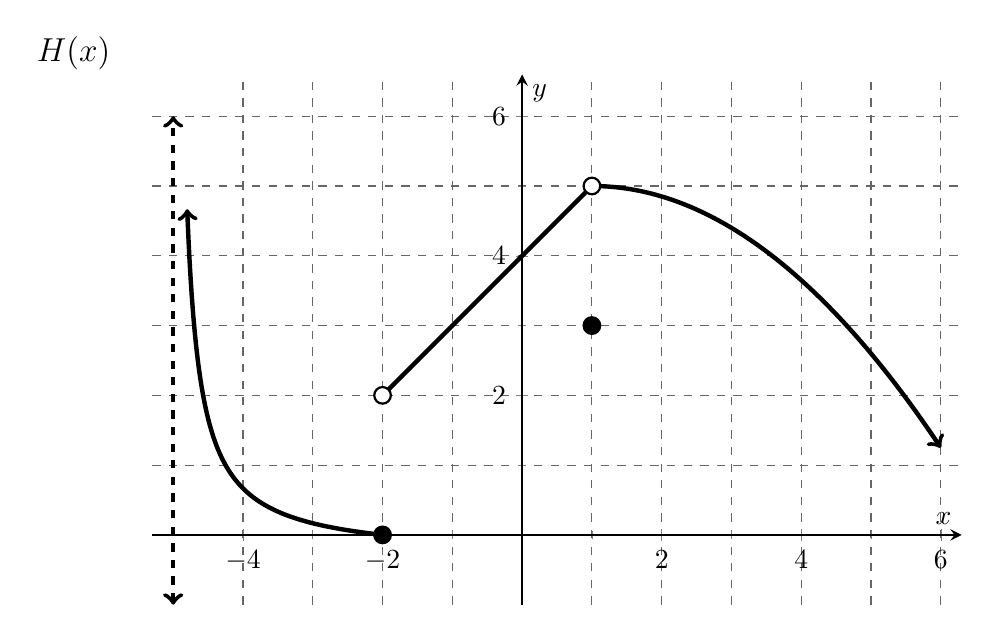
\begin{tikzpicture}
\begin{axis}[scale=1.5, thick, my style, xtick={-4,-2,...,6}, ytick={0,2,...,6},
xmin=-5.3, xmax=6.3, ymin=-1, ymax=6.6, minor y tick num=1,
        minor x tick num=1, mark size=3.0pt, grid=both, grid style={ thin, black!60, dashed}, axis equal image]
% %%asymptote
\addplot[dashed,<->, ultra thick] coordinates {(-5,-1) (-5,6)};       
%%points solid
\addplot[mark=*,only marks] coordinates {(-2,0)(1,3)};
%%points open
\addplot[mark=*,fill=white,only marks] coordinates {(-2,2)(1,5)};
%%Curves
\addplot[<-,ultra thick, smooth, variable=\x, samples=100, domain=-4.8:-2] plot(\x,{1/(\x+5) - 0.333});
\addplot[ultra thick, smooth] coordinates {(-2,2) (1,5)};
 \addplot[->,ultra thick, smooth, variable=\x, samples=100, domain=1:6] plot(\x,{(-0.15)*(\x -1)*(\x -1)+5});    
\end{axis}
\node at (-1,7){\large{$H(x)$}};
\end{tikzpicture}
\end{center}

\begin{enumerate}
\begin{multicols}{3}
\item $H(-2)=\mblank{.5in}$
\item $H(1)=\mblank{.5in}$
\item $\d{\lim_{x \to\; -2^+} H(x)=\mblank{.5in}}$
%\item $f(5)=\mblank{.5in}$
\end{multicols}
\vspace{0.1in}
\begin{multicols}{3}
\item $\d{\lim_{x \to\; -2} H(x)=\mblank{.5in}}$
\item $\d{\lim_{x \to\; -5^+} H(x)=\mblank{.5in}}$
\item $\d{\lim_{x \to\; 1} H(x)=\mblank{.5in}}$
\end{multicols}
\vspace{0.1in}
\item Estimate $H(4).$
\vspace{0.1in}
\item Evaluate $\d{\lim_{x \to\; 0} ( 5H(x) +2)}.$
\vspace{0.1in}
\item List all $x$-values in the domain of $H(x)$ for which the function $H(x)$ fails to be continuous.\\
\vfill

\end{enumerate}

\item (3 points)  If $\d \lim_{x \to -2} f(x) =3$ and $\d \lim_{x \to -2} g(x) =5$, is it possible to evaluate $\d \lim_{x \to -2} \frac{f(x) +1}{xg(x)}$? If so evaluate the limit. If not, explain why.
\vspace{1in}

\newpage

\item (8 points) Use algebra to evaluate the limits below. You must show your work to earn full credit \emph{and} your work will be graded. (That is, you need to write your mathematics correctly.)
	\begin{enumerate}
	\item $\d \lim_{x \to \sqrt{7}} \frac{x-\sqrt{7}}{x^2-7}=$
	\vfill
	\item $\d \lim_{h \to 0} \frac{(a+h)^2-a^2}{h}=$
	\vfill
	\end{enumerate}
\item (4 points) Let $f(x)=\begin{cases} 2-x^2 & x < 0\\e^x & x \geq 0 \end{cases}.$ 
\begin{enumerate}
	\item Find $\d \lim_{x \to 0^-} f(x).$
	\vspace{.7in}
	\item Find $\d \lim_{x \to 0^+} f(x).$
	\vspace{.7in}
	\item Use your answers to parts (a) and (b) to justify whether $f(x)$ is or is not continuous at $x=0.$ (Your answer should be a complete sentence.)
	\vspace{.7in}
\end{enumerate}
\end{enumerate}
\end{document}